\documentclass[a4paper, 12pt]{scrreprt}
\usepackage[german]{babel}
\usepackage[german]{translator}
\usepackage[utf8]{inputenc}
\usepackage[T1]{fontenc}
\usepackage{ae}
\usepackage[bookmarks,bookmarksnumbered]{hyperref}
\usepackage{graphicx}
\usepackage{scrpage2}
\usepackage{color}
\usepackage{appendix}
\usepackage[dvipsnames]{xcolor}
\usepackage{booktabs}
\usepackage{longtable}
\usepackage{listings}
\usepackage{tabularx}
\usepackage[left=2.00cm, right=2.50cm, bottom =3.53cm]{geometry}
\usepackage{ pdflscape}
%\usepackage{pdfpages}
%\usepackage[section]{placeins}


\newcommand{\col}[2]{\textcolor{#1}{#2}}

% Zeilenhöhe bei Tabellen
\newcommand{\zh}[1]{\parbox[0pt][#1][c]{0cm}{}}

\begin{document}
	\thispagestyle{plain}

\begin{titlepage}
    \begin{center}
        \begin{figure}[ht]
            \centering
            
\includegraphics[width=0.66\textwidth, angle=0]{logo/name_blau_ofCourse.jpg}
        \end{figure}

    	\begin{title}
        	\title{\Huge{\textbf{Kurseinheiten-Manager \\ Validierungsbericht\\}}}

		\end{title}
		\hspace{3cm}

        	Software Engineering Praktikum \\
        	Sommersemester 2015\\
        	Universität Passau\\


        	Betreuer: Andreas Stahlbauer \\
        	\hspace{1,5cm}\\
        	Version: 1.0 \\
        	\hspace{1,5cm}\\
        	Datum: 03.07.2015\\[50pt]
        	Team 3 \\
    
		    \ \\
        
        \begin{tabular}{ | l | l | l | l |}
        	\hline
        	\textbf{Matrikelnummer} & \textbf{Name} & \textbf{Phase} & \textbf{E-Mail}  \\ \hline
        	63097 & Katharina Hölzl & Pflichtenheft & hoelzlka@fim.uni-passau.de \\ \hline
        	64504 & Ricky Strohmeier& Entwurf & strohric@fim.uni-passau.de  \\ \hline
        	61085 & Sebastian Schwarz & Feinspezifikation & sebastian@nrschwarz.de \\ \hline 
        	64080 & Tobias Fuchs & Implementierung  &  fuchstob@fim.uni-passau.de\\ \hline
        	58379 & Patrick Cretu  &  Validierung & cretu@fim.uni-passau.de \\ \hline
        \end{tabular}
        
        \ \\
        \ \\
       
        \hspace{3 cm}\\
         \textbf{Arbeitspakete Validierung} \\
         \ \\
         
         \begin{tabular}{ | l | l |}
         	\hline
         	\textbf{Autor} & \textbf{Verantwortungsbereich} \\ \hline
         	Katharina Hölzl & Pflichtenhefttests\\ \hline
         	Ricky Strohmeier& Pflichtenhefttests, Usability-Tests \\ \hline
         	Tobias Fuchs & Pflichtenhefttests, Usability-Tests \\ \hline
         	Sebastian Schwarz & Pflichtenhefttests, Last-Tests, Code Coverage \\ \hline  
         	Patrick Cretu  &  Pflichtenhefttests, Last-Tests  \\ \hline
         \end{tabular}       
       
       
        
        
    \end{center}
\end{titlepage}


% Platzierung des Inhaltsverzeichnisses
\tableofcontents


\chapter{Einleitung}
\begin{tiny}
MB \\
\end{tiny}
In diesem Dokument wird der grundlegende Entwurf der Webanwendung \glqq ofCourse\grqq{} dargestellt. Diese Webapplikation soll es Betreibern verschiedensten Fachbereichen erleichtern ihre Veranstaltungen zu organisieren, sowie zu planen. Des Weiteren können sich Nutzer von \glqq ofCourse\grqq{} über jene Veranstaltungen bzw. Kurse leicht informieren und anmelden. Im Laufe dieses Dokuments wird auf die Architektur des Systems, die verwendeten Design Patterns und die Fehlerbehandlungen eingegangen. Im Klassendiagramm werden die einzelnen Klassen des Systems, sowie die Pakete präsentiert. Eine genauere Erklärung der View wird im Kapitel der Facelets und deren jeweiligen Elemente diskutiert. In den Systemfunktionen werden grundlegende Aktionen, wie Email-Versand erläutert, sowie der Umgang mit Fehlern. Zum besseren Verständnis des Datenfluss wird jeweils ein Sequenzdiagramm bezüglich einer typischen Aktion in der Applikation veranschaulicht. 
Am Ende dieser Entwurfsbeschreibung wird das verwendete Datenbankschema mithilfe eines ER-Modells graphisch dargestellt.

\chapter{Tests aus dem Pflichtenheft}

\begin{landscape}
	\section{Testfälle für den Systemadministrator ohne bestehenden Datensatz}	
		\begin{tabular}{|p{2.0cm} |p{5.0cm}|p{3.0cm}|p{5.0cm}|p{4.0cm}|p{4.0cm}|}
			\hline \textbf{Testnr. (Tester)} & \textbf{Bezeichnung} & \textbf{Ergebnis} & \textbf{Ursache} & \textbf{Ergebnis} & \textbf{Ursache} \\ 
      	    \hline    T10-10   &      AuthenticationTest (zusätzlich werden Fehlerfälle geprüft, die bei der Anmeldung auftreten können)   &  erfolgreich &                  &                   &                  \\ 
      	    
      	     \hline    T10-30 (TF)  &    OverdraftCreditAdminTest: In diesem Test wird die Funktionalität der Änderung des Überziehungskredits durch den Admin getestet.
      	                             Zustätzlich zum wurden noch mehr Fehlerfälle getestet   &  fehlgeschlagen &    negative Werte wurden akzeptiert, Eingabeformat kompliziert, falsche Interpretation von z.b. 10.00 als 1000              &      erfolgreich             &                  \\ 
      	                             
      	    \hline    T10-40 (TF)   &    ActivationTypeAdminTest: In diesem Test wird die Funktionalität der Änderung des Typs der Accountaktivierung durch den Admin getestet.
      	      &  erfolgreich &             &                &                  \\                          
      	                             
			
			\hline T10-80, T10-90   &      CreateCourseTest  (Das Anlegen der Kurse aus den beiden Testfällen wird in einer Testklasse durchgeführt. Beide Kurse werden angelegt, zusätzlich wird auf weitere Fehlerfälle geprüft)              &      erfolgreich             &                  &                   &                  \\ 
			\hline       &          &          &        &         &       \\
			\hline 
		\end{tabular} \ \\
		\ \\
	\section{Testfälle für den Kursleiter}
		\begin{tabular}{|p{2.0cm} |p{5.0cm}|p{3.0cm}|p{5.0cm}|p{4.0cm}|p{4.0cm}|}
			\hline \textbf{Testnr.} & \textbf{Bezeichnung} & \textbf{Ergebnis} & \textbf{Ursache} & \textbf{Ergebnis} & \textbf{Ursache} \\
			\hline       &          &          &        &         &       \\
			\hline       &          &          &        &         &       \\
			\hline       &          &          &        &         &       \\
			\hline       &          &          &        &         &       \\
			\hline 
		\end{tabular} \ \\
		\ \\
				
	\section{Testfälle für anonymer Benutzer}
		\begin{tabular}{|p{2.0cm} |p{5.0cm}|p{3.0cm}|p{5.0cm}|p{4.0cm}|p{4.0cm}|}
			\hline \textbf{Testnr.} & \textbf{Bezeichnung} & \textbf{Ergebnis} & \textbf{Ursache} & \textbf{Ergebnis} & \textbf{Ursache} \\
			\hline   T30-30    & RegistrationTest (zustätzlich werden weitere Fehlerfälle geprüft, die bei der Registrierung auftreten können)   &   fehlgeschlagen       &    Die E-Mail-Adresse 'Katharina\_hoelzl@web.de wurde akzeptiert, obwohl katharina\_hoelzl@web.de bereits in der Datenbank vorhanden war. Verbesserung in der RegisterUserBean: Mail wird nun zu lower case konvertiert.    &    erfolgreich     &       \\
			\hline       &          &          &        &         &       \\
			\hline       &          &          &        &         &       \\
			\hline       &          &          &        &         &       \\
			\hline 
		\end{tabular} \ \\
		\ \\
			
	\section{Testfälle für den registrierten Benutzer}
		\begin{tabular}{|p{2.0cm} |p{5.0cm}|p{3.0cm}|p{5.0cm}|p{4.0cm}|p{4.0cm}|}
			\hline \textbf{Testnr.} & \textbf{Bezeichnung} & \textbf{Ergebnis} & \textbf{Ursache} & \textbf{Ergebnis} & \textbf{Ursache} \\
			\hline T40-10   &  UserNotYetActivatedTest        & erfolgreich   &        &         &       \\
			\hline T40-20   & AccountActivationByAdmin Test  & erfolgreich    &        &         &       \\	
			\hline T40-70   & SignUpForCourseYogaTest & erfolgreich &        &         &       \\	
			\hline T40-140  & HelpTest & erfolgreich &        &         &       \\	
			\hline T40-200  & LogoutTest & erfolgreich &        &         &       \\	
			\hline       &          &          &        &         &       \\
			\hline 
		\end{tabular} \ \\
		\ \\
			
	\section{Testfälle mit Datensatz}	
		\begin{tabular}{|p{2.0cm} |p{5.0cm}|p{3.0cm}|p{5.0cm}|p{4.0cm}|p{4.0cm}|}
			\hline \textbf{Testnr.} & \textbf{Bezeichnung} & \textbf{Ergebnis} & \textbf{Ursache} & \textbf{Ergebnis} & \textbf{Ursache} \\
			\hline  T40-180, T50-40  & ListParticipantsTest (Die beiden Testfälle 'Teilnehmer ansehen' und 'Teilnehmer aus Kurs entfernen' wurden in eine Testklasse zusammengefasst.) &     erfolgreich     &        &         &       \\
			\hline  T50-50  &  AddLeaderToCourseTest (zusätzlich wurden Fehlerfälle geprüft) &  fehlgeschlagen & Es wurde bei der Eingabe der KursleiterID nicht geprüft ob die ID zu einem Kursleiter gehört. Behebung des Fehlers durch hinzufügen des Validators CourseInstructor zum Facelet CourseDetail.xhtml  &  erfolgreich       &       \\
			\hline       &          &          &        &         &       \\
			\hline       &          &          &        &         &       \\
			\hline       &          &          &        &         &       \\
			\hline 
		\end{tabular} \ \\
		\ \\
	
\end{landscape}
\chapter{Usability - Tests}
Um das \textbf{ofCourse} System bezüglich dem Gesichtspunkt der Benutzbarkeit bzw. der Benutzerfreundlichkeit zu testen,
wurden unvoreingenommene Testpersonen gesucht, welche das System testeten und anschließend das System, aufgrund der
während der Tests gewonnenen Eindrücke evaluierten.

\subsection{Durchführung}

\subsection{Material}

\subsection{Ergebnisse}

\subsection{Frage 1}

\subsection{Frage 2}

\subsection{Frage 3}

\subsection{Frage 4}

\subsection{Frage 5}

\subsection{Bearbeitungszeit}

\subsection{Anregungen/Verbessungsvorschläge}

\subsection{Fazit}
\chapter{Lasttests}
\chapter{Code Coverage}
\begin{tiny}
	SS
\end{tiny}


Um den Code Coverage unseres Systems \textbf{OfCourse} zu testen, benutzten wir das Java Plugin ECLEmma und führten alle Tests mithilfe einer JUnit TestSuit auf einmal aus.
Es ist uns leider nicht gelungen, dass ECLEmma auf den Code zugreifen kann. Dadurch, dass unsere JUnit Tests mit einem WebDriver laufen erkannt er nicht welche Methoden im Hintergrund ausgeführt worden sind. 
Dies sieht man sehr deutlich an dem Ergebnis.

\begin{figure}[h]
\centering
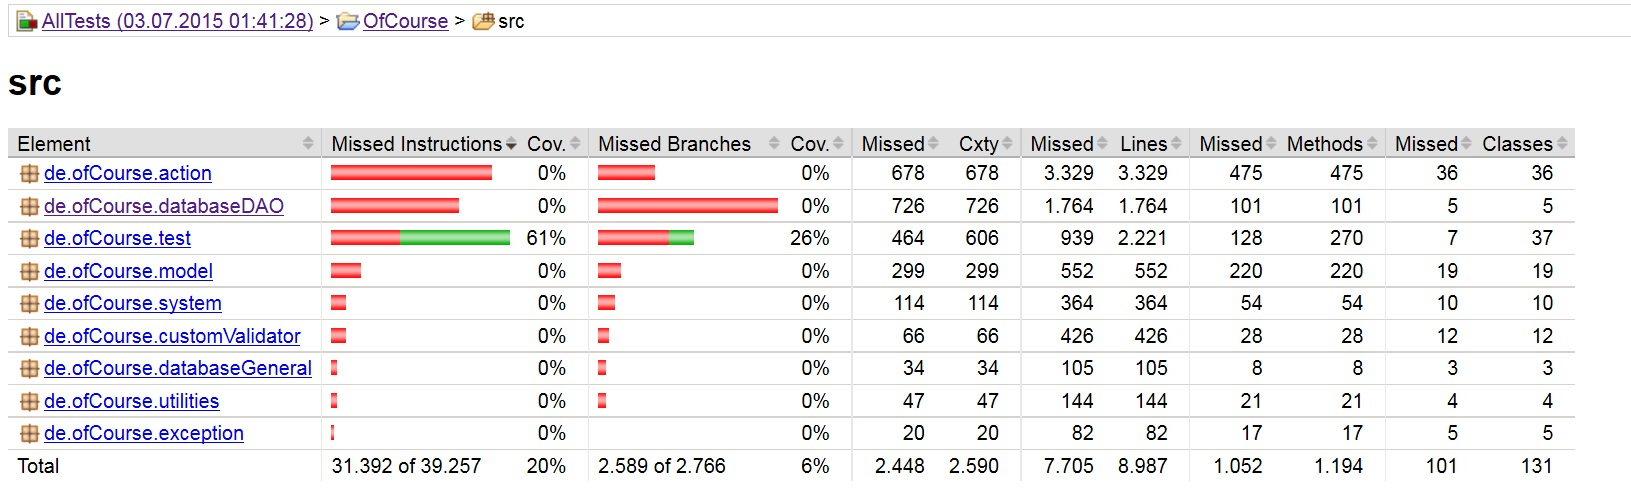
\includegraphics[width=1\linewidth]{img/CodeCoverage}
\caption{CodeCoverage}
\label{fig:CodeCoverage}
\end{figure}

\appendix
\pagestyle{scrheadings}
\clearscrheadfoot
\chapter{Anhang}
\ihead{\textbf{Anhang 1: Feedback - Fragebogen ofCourse}}
\begin{figure}[h]
\centering
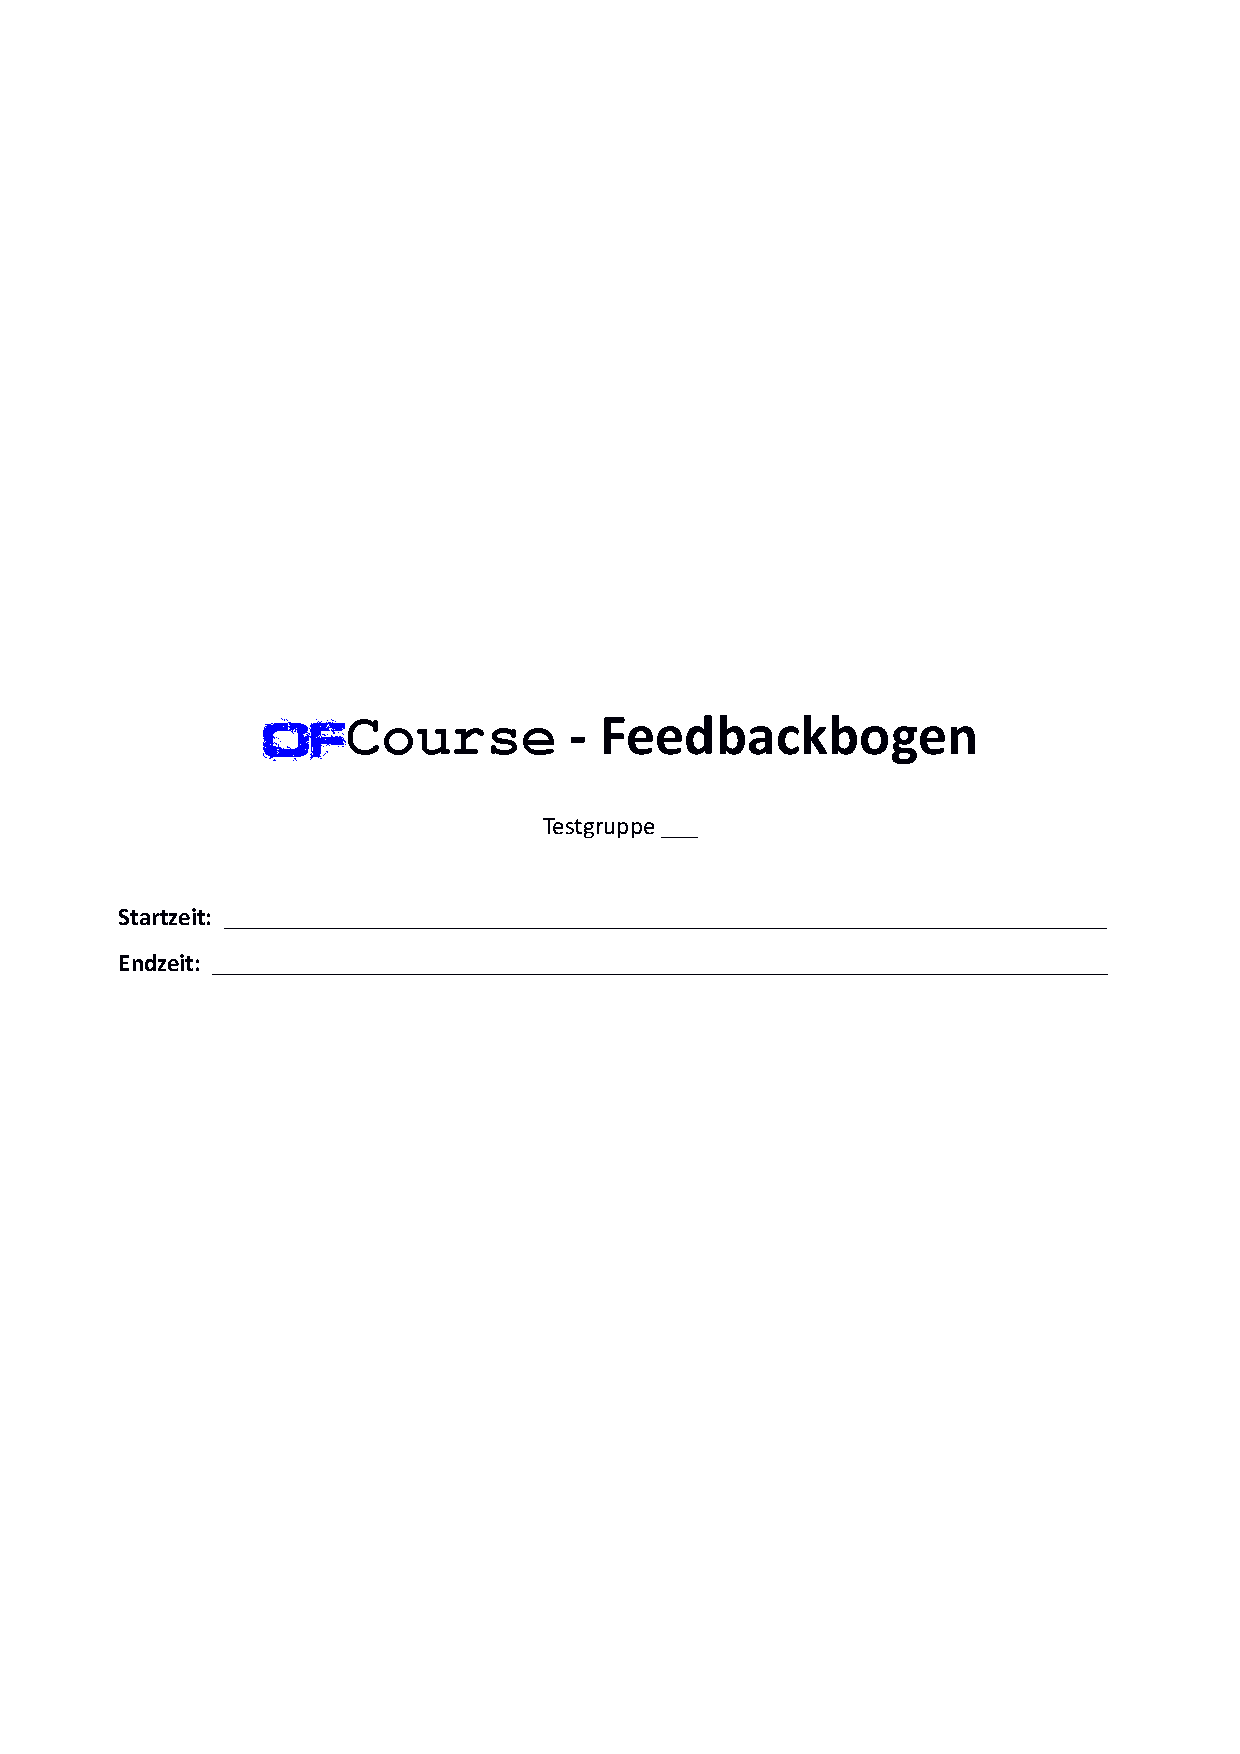
\includegraphics[width=0.9\linewidth, page=1]{pdf/OfCourseFeedback}
\label{fig:OfCourseFeedback}
\end{figure}
\begin{figure}
	\centering
	\includegraphics[width=0.9\linewidth, page=2]{pdf/OfCourseFeedback}
	\caption{Feedback - Fragebogen ofCourse}
\end{figure}
\ihead{\textbf{Anhang 2: Arbeitsanweisungen Testgruppe 1}}
\begin{figure}[h]
	\centering
	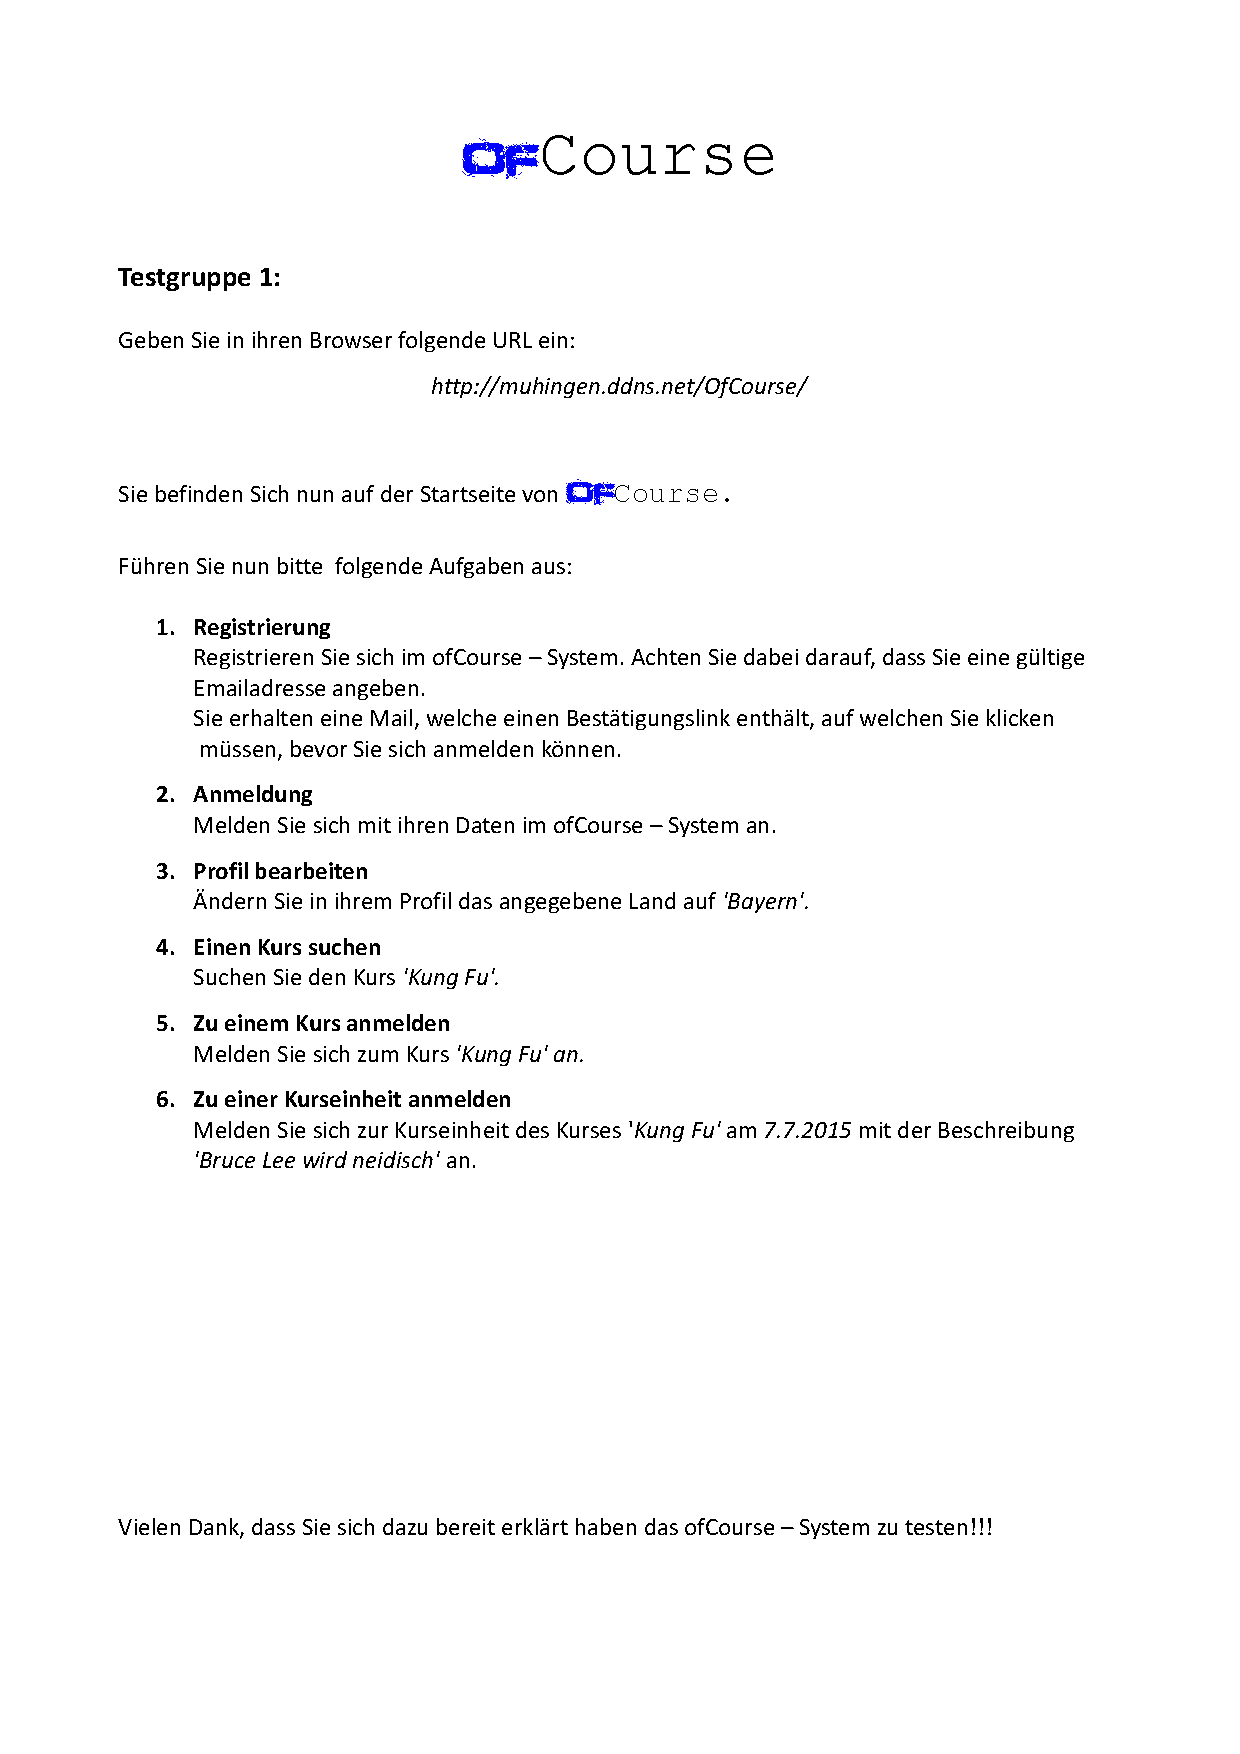
\includegraphics[width=0.9\linewidth, page=1]{pdf/AnweisungenTestgruppe1}
	\caption{Anweisungen Testgruppe 1}
	\label{fig:Anweisungen1}
\end{figure}
\ihead{\textbf{Anhang 3: Arbeitsanweisungen Testgruppe 2}}
\begin{figure}[h]
	\centering
	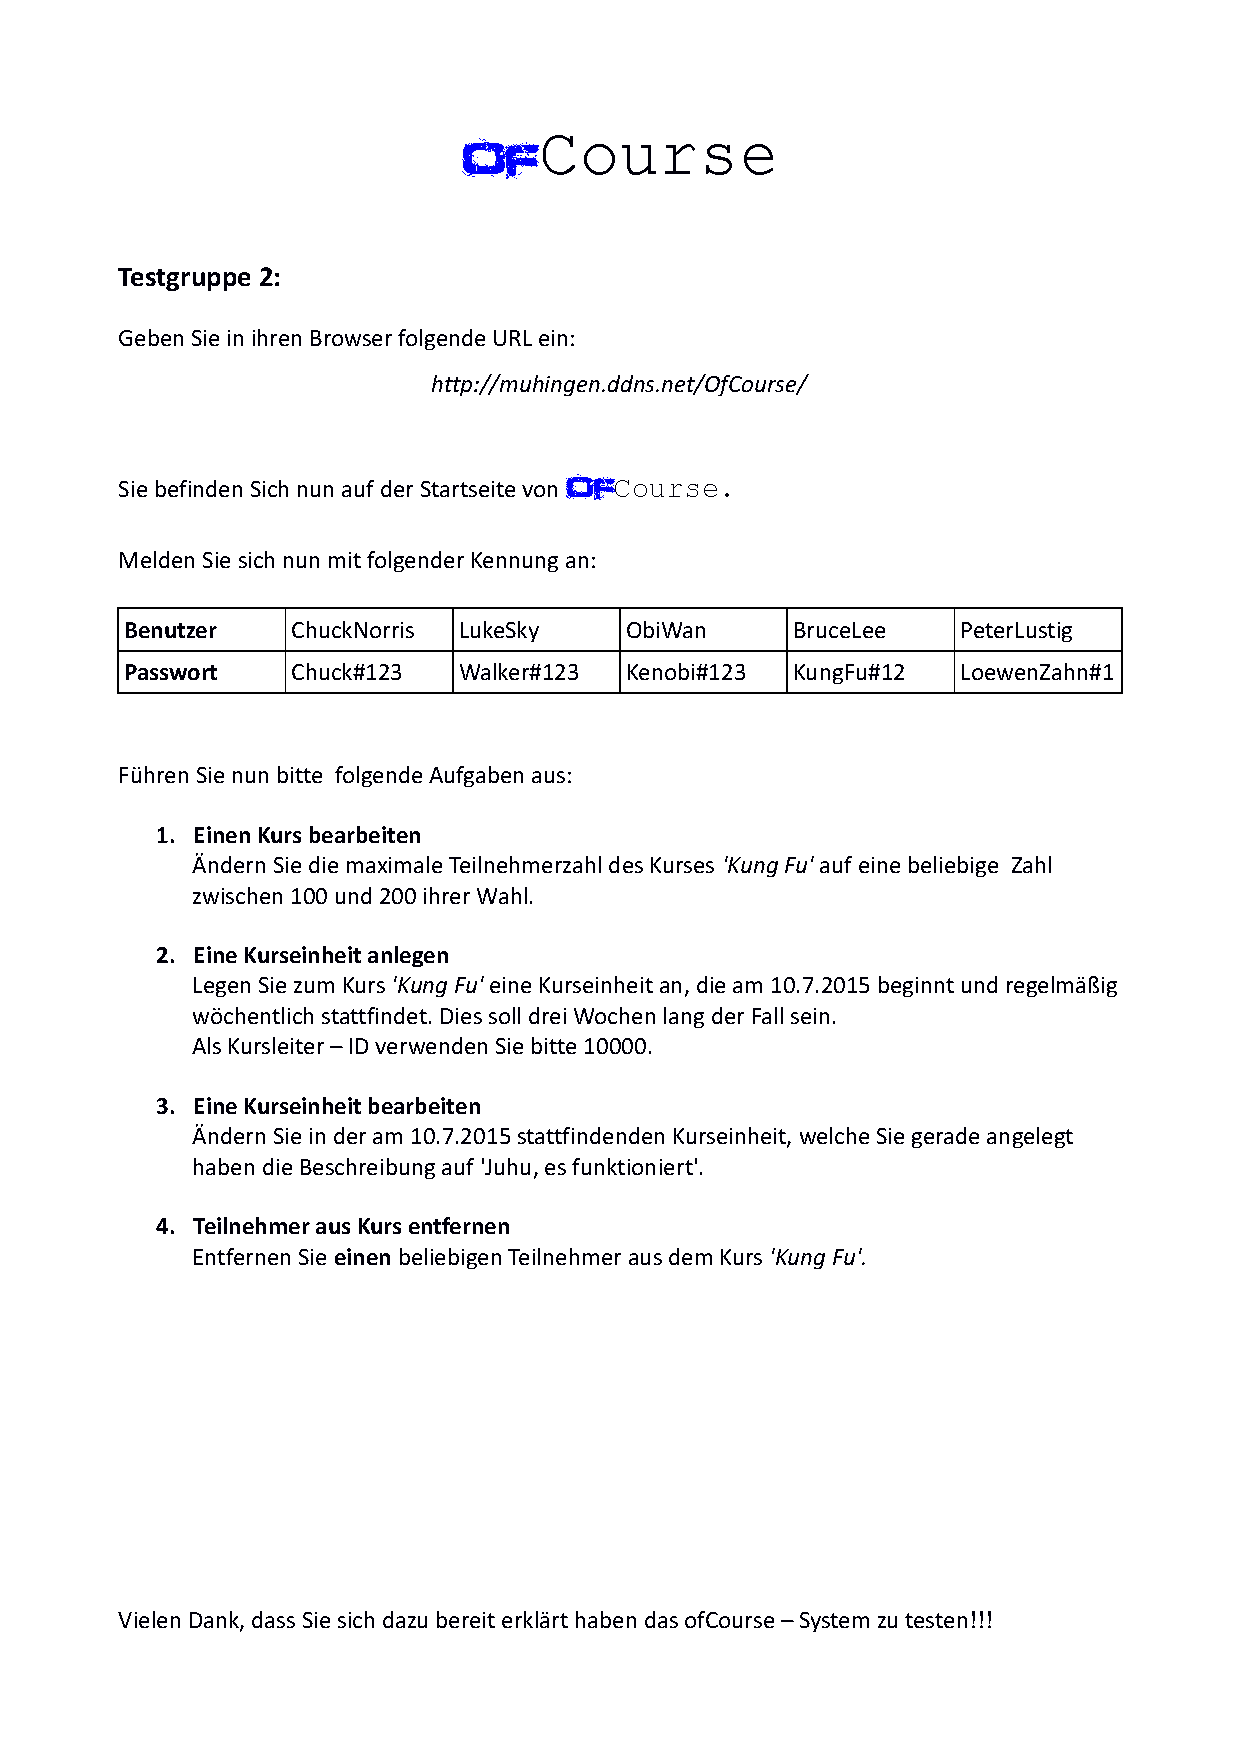
\includegraphics[width=0.9\linewidth, page=1]{pdf/AnweisungenTestgruppe2}		\caption{Anweisungen Testgruppe 2}
	\label{fig:Anweisungen2}
\end{figure}
\ihead{\textbf{Anhang 4: Arbeitsanweisungen Testgruppe 3}}
\begin{figure}[h]
	\centering
	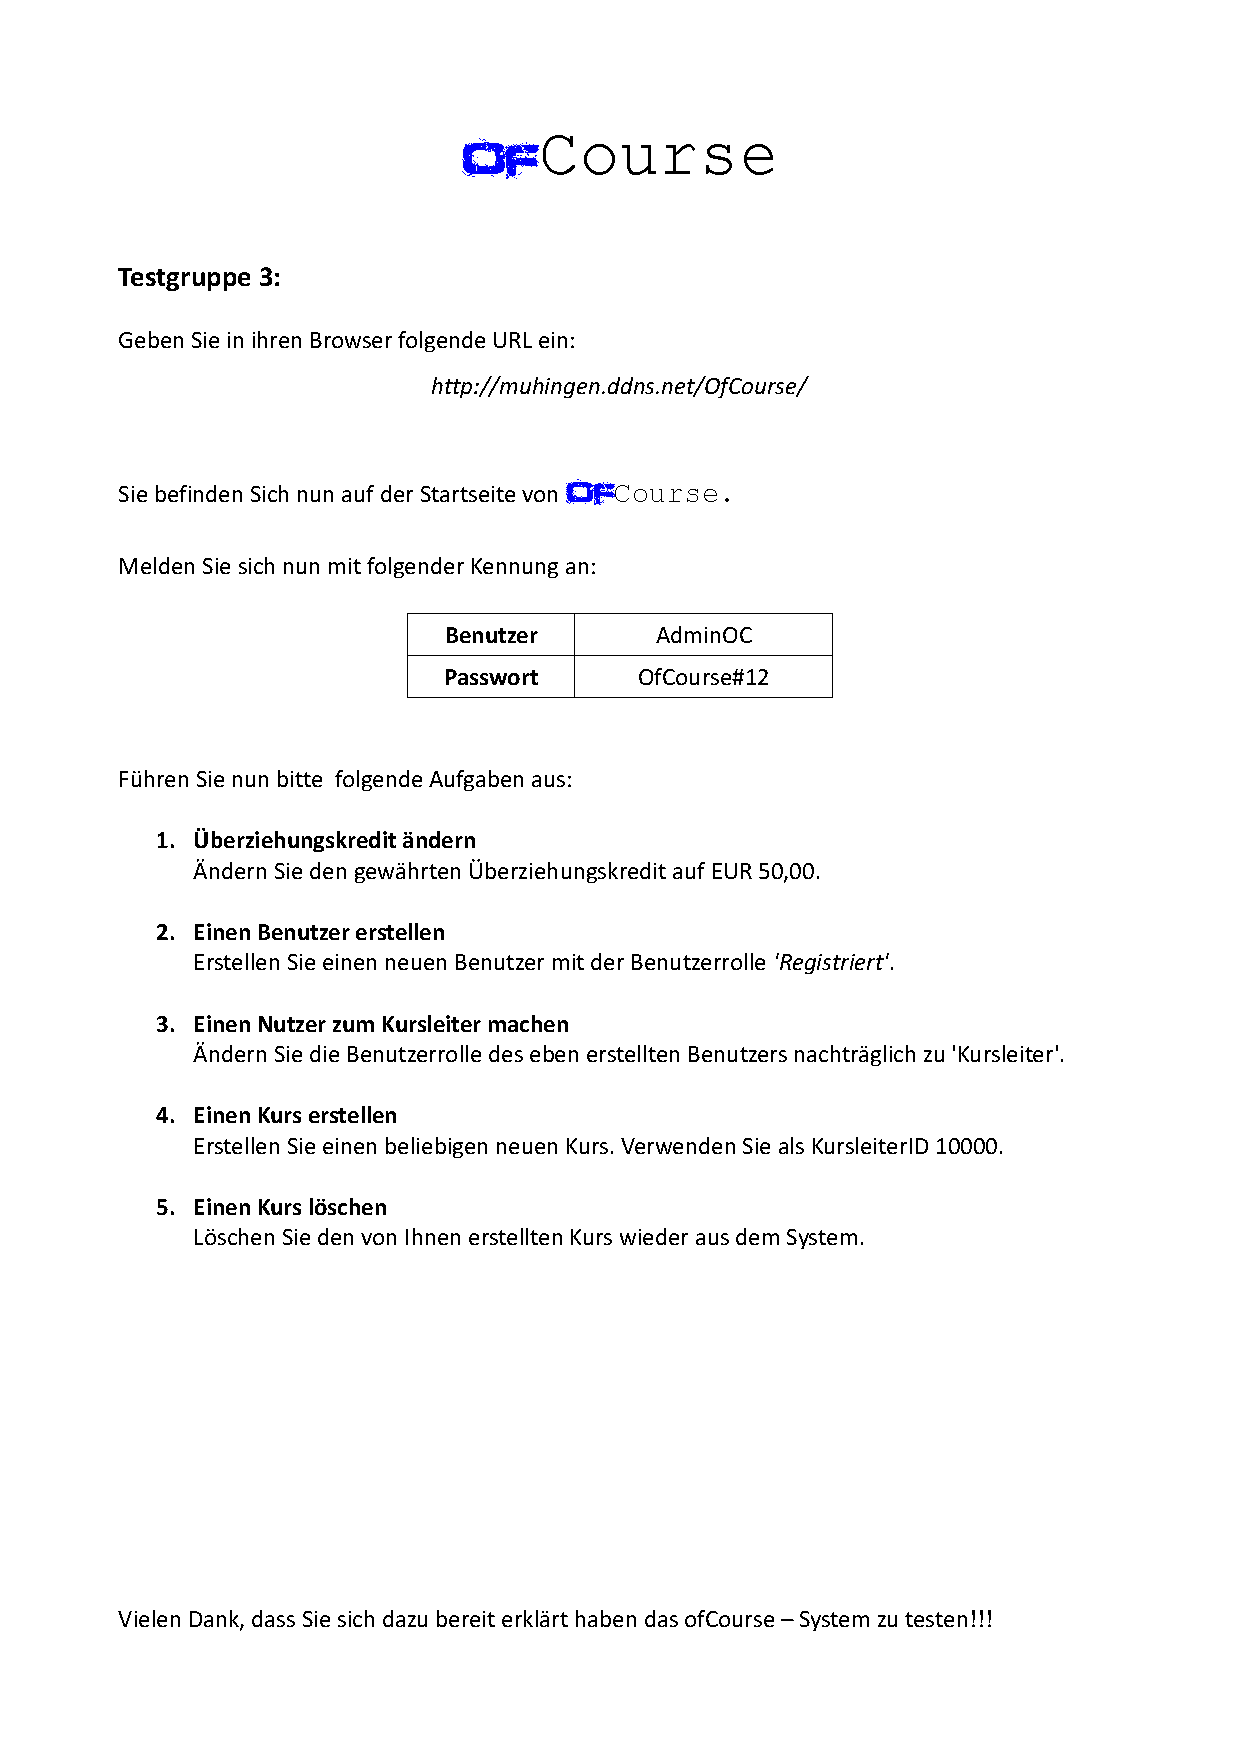
\includegraphics[width=0.9\linewidth, page=1]{pdf/AnweisungenTestgruppe3}
	\caption{Anweisungen Testgruppe 3}
	\label{fig:Anweisungen3}
\end{figure}
\end{document}